\documentclass[12pt,a4paper,titlepage]{article}
\usepackage[utf8]{inputenc}
\usepackage[T1]{fontenc}
\usepackage{amsmath}
\usepackage{amsfonts}
\usepackage{amssymb}
\usepackage[left=3cm,right=3cm,top=2.5cm,bottom=2.5cm]{geometry}
\usepackage[dvipsnames]{xcolor}
\usepackage[czech]{babel}
\usepackage[
  backend=biber,
  style=iso-numeric,
  maxbibnames=99
]{biblatex}
\addbibresource{maturitni_prace.bib}
\usepackage{graphicx}
\usepackage{minted}
\usepackage{subcaption}
\usepackage{tikz}
\usepackage{pgfplots}
\pgfplotsset{compat=1.18}
\graphicspath{ {./images/} }
\usepackage{indentfirst}
\usepackage{setspace}
\fontfamily{ptm}
\usepackage{tabularx,ragged2e,booktabs}
\usepackage{hyperref}
\usepackage{csquotes}
\usepackage{xurl}

\DeclareBibliographyCategory{skipbibliography}
\DeclareCiteCommand{\fcite}[\mkbibfootnote]
  {\usebibmacro{prenote}}
  {\addtocategory{skipbibliography}{\thefield{entrykey}}%
   \usedriver{\DeclareNameAlias{sortname}{default}}{\thefield{entrytype}}}
  {\multicitedelim}
  {\usebibmacro{postnote}}

\author{Antonín Vřešťál}
\title{Tvorba astronomických videí}
\renewcommand{\baselinestretch}{1.5} 


\begin{document}
\begin{titlepage}
	\begin{center}
		Waldorfská základní a~střední škola Semily, p.\  o.\\
		Tyršova 485, 513 01 Semily
		\vspace*{1cm}
 
		\vfill		

		\Huge
		Tvorba astronomických videí
 
		\normalsize
		\vspace{0.5cm}
		Maturitní práce 	 
		 
		\vfill		
	\end{center}
	Vypracoval: Antonín Vřešťál\\
	Vedoucí práce: MgA. Mojmír Dlabola\\
	\textcolor{red}{Pracovní verze}\\
 \end{titlepage}
\newpage
\section*{Prohlášení}
Prohlašuji, že jsem tuto projektovou maturitní práci \enquote{Tvorba astronomických videí} napsal samostatně a~výhradně s~použitím citovaných pramenů. Souhlasím, aby má projektová maturitní práce byla zpřístupněna veřejnosti ke studijním účelům.
\section*{Poděkování}
Děkuji MgA. Mojmíru Dlabolovi, vedoucímu mé práce, za podnětné připomínky k~projektové maturitní práci po stránce obsahové i~stylistické a~za doporučení vhodné a~zajímavé literatury. Velmi si vážím času, který věnoval vedení mé práce.\\
\\
V Semilech dne \hspace{0.05cm} \rule[-3pt]{1.5in}{0.5pt}\\
\\
\hspace{0.5cm} \rule[-3pt]{5.5cm}{0.5pt}\\
\indent \indent Antonín Vřešťál\\

\newpage
\tableofcontents
\newpage
\part{Teoretická část}
\section{Úvod}
%\textcolor{red}{(Nejsem si úplně jistý, jak by měla tato sekce vypadat, budu rád za Váš názor.)}
Tvorbou astronomických videí se zabývám více než tři roky, a~to jako editor ve skupině AstroCrew. Skupinu AstroCrew tvoří tři členové:

\begin{itemize}
	\item Daniel Kurtin píše scénáře,
	\item Terka Toušová načítá text na mikrofon
	\item Já (Antonín Vřešťál) k~nahrávkám následně tvořím grafický podklad a~kompletuji veškerá data do výsledného videa.
\end{itemize}
Hotová videa následně publikujeme na našem YouTube kanálu. 

Základním cílem skupiny AstroCrew je zpřístupnit široké veřejnosti zajímavé úkazy na obloze pomocí animací a~videí. Diváci mají poté lepší přehled o~umístění jednotlivých úkazů na noční obloze a~mohou je následně lépe nalézt.

Spolupracujeme s~planetáriem v~liberecké iQLandii. Na jejich akcích \enquote{Večery pod hvězdami} jsou naše nová videa promítána přímo v~planetáriu jako součást oficiálního programu. Kromě videí o~astronomii zpřístupňujeme široké veřejnosti i~kosmonautiku. V~tomto odvětví se věnujeme primárně živým přenosům startů raket, poslední dobou nejvíce programu Starship.

Téma tvorby astronomických videí jsem si vybral zejména kvůli jeho obsáhlosti. V~rámci produkce videí ve skupině AstroCrew programuji animační nástroje, ale následně pomocí nich animuji scénu a~výsledná data nakonec kompletuji ve finální video. V~této maturitní práci se zaměřuji zejména na moji část produkce videa. Ostatní části tvorby videa, které nezpracovávám já, jsou zastoupeny pouze stručně obsahově pro doplnění kontextu. 
\section{Postup vytváření videa}\label{makingof}
\subsection{Příprava textových a~zvukových podkladů}\label{makingof:text-audio-prep}
Téma připravovaného videa je většinou rozhodnuto s~dostatečným předstihem na základě společném diskuze. Každé video je unikátní s~ohledem na námi zvolené požadavky. Tyto požadavky vybíráme na základě chyb, nedostatků a~nových zjištění nabytých při tvorbě předchozích videí. V~případě videa, týkajícího se úkazů na noční obloze v~roce 2025, byla hlavním tématem diskuze o~jeho délce s~ohledem na rozhodnutí, které úkazy do videa budou zahrnuty a~které bude nutno vynechat.

Dalším krokem v~produkci videa je sepsání scénáře naším scénáristou Danem Kurtinem. 

Po dokončení scénáře jde na řadu samotné nahrávání audiostopy. Proces nahrávání je odlišný pro každý samostatný projekt. Pro obě videa, řešená touto projektovou maturitní prací, byl proces tvorby zvuku víceméně shodný, až na malé detaily. 

\textcolor{red}{Zeptat se terky na popis studia doma i~v Praze}

Terka standardně nahrává audiostopy v~domácím nahrávacím studiu. Tentokrát byla nucena z časových důvodů nahrávat audiostopu na mobilní telefon na kolejích v~Praze. Kombinace těchto faktorů způsobila, že prosincové video obsahuje výrazný šum na pozadí nahrávky, který není možné úplně odstranit. Tento problém se nám podařilo vyřešit v~následujícím videu pomocí \enquote{peřinového bunkru}, který značnou část šumu na pozadí odfiltroval. I~bez speciálních zvukových panelů, které jsou pro tento účel instalovány ve studiích, se nám podařilo výrazně zvýšit kvalitu zvukové stopy. Porovnání šumu na zvukových stopách je znázorněno frekvenční analýzou na obrázku níže.
\begin{figure}[h]
	\centering
	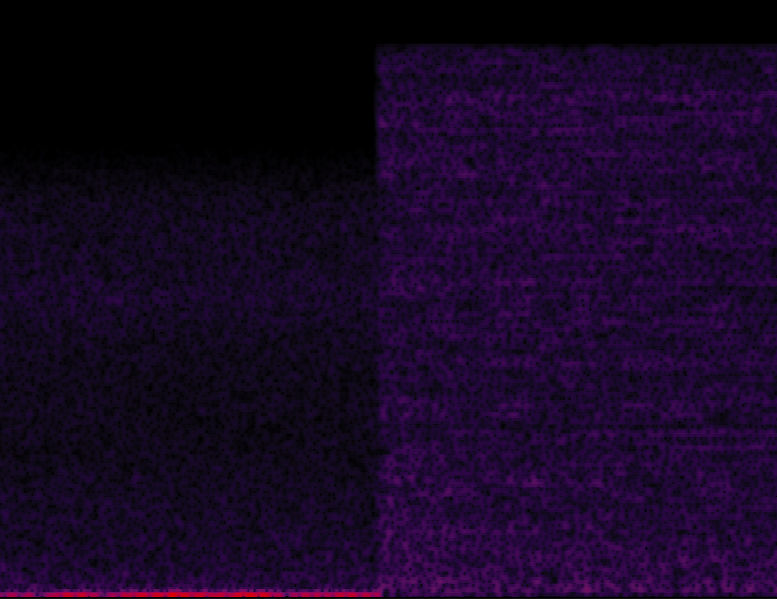
\includegraphics[width=.4\textwidth]{fourier.png}
	\caption{Porovnání šumové stopy projektu Rok 2025 (vlevo, využit \enquote{peřinový bunkr} pro snížení hladiny šumu) a~projektu Prosinec (vpravo).}\label{img:fourier}
\end{figure}
\subsection{Animování oblohy v~programu Stellárium}\label{makingof:stellarium}
Celý proces animování začíná prací se scénářem. Ze scénáře se vypíše seznam jednotlivých scén a~přechodů mezi nimi. Pro tento úkol jsem si vytvořil speciální formát zápisu, který obsahuje vše, co je potřebné k~vytvoření jednotlivých přechodů ve videu. Viz tabulka níže.

\begin{table}[h]
	\centering
	\begin{tabularx}{\linewidth}{lc*{5}{>{\RaggedRight\arraybackslash}X}}
	\toprule
	\# scény    & Směr scény & Čas          & Souhvězdí         & Speciální objekty      \\ \midrule
	0000        & Z obzor    & západ slunce & Labuť, Lyra, Orel & Letní trojúhelník      \\ \addlinespace
	0001        & SZ obzor   & západ slunce & dtto, Herkules    & Herkulův květináč, M13 \\ \addlinespace
	0002        & Z obzor    & západ slunce & dtto              & ---                    \\ \addlinespace
	\ldots      & \ldots     & \ldots       & \ldots            & \ldots                 \\ \bottomrule
	\end{tabularx}
	\caption{Demonstrace tabulky s~informacemi o~scénách}\label{tab:scenar}
\end{table}		

Většina animací, které se v~těchto videích nachází, byly vytvořeny pomocí simulačního programu Stellarium. Tento program je open-source (jeho zdrojový kód je volně dostupný) a~jeho primárním účelem je realistická simulace noční oblohy při pohledu očima nebo dalekohledem\fcite{stellarium:homepage}. Stellarium poskytuje širokou nabídku programovatelných rozhraní. Pro účely této práce využívám webový server, přes který lze instanci Stellaria ovládat z prohlížeče a~skriptovací rozhraní, které umožňuje interakci se Stellariem pomocí programovacího jazyka, založeného na standardu ECMAScript (využívaného například jazykem JavaScript\fcite{wiki:ecmascript}).

Největším problémem pro využití Stellaria v~produkci videí je fakt, že jeho tvůrci nepočítali s~jeho využitím pro tvorbu videí. Neexistuje tam například funkce, která by Stellariu řekla \enquote{Otoč se plynule na tyto souřadnice a~přitom nahraj video}. Jedinou možností, jak získat tuto animaci, je export každého samostatného snímku jako separátního souboru a~tyto jednotlivé snímky následně spojit do finálního videa pomocí nástroje jako FFmpeg. 

Prvním krokem v~tomto procesu je získání souřadnic jednotlivých snímků. Zatím jediná data, která máme jsou souřadnice, přiblížení, datum a~čas pro začátek a~konec přechodu. Tyto data je možné zabalit do vektoru $\vec{s}$ a~$\vec{e}$, které značí hodnotu začátku a~konce přechodu v~pětidimenzionálním prostoru. 5D prostor je velice obtížné si představit, proto ho nachvíli zjednodušíme do 2D prostoru, kde jedna dimenze bude představovat azimut a~druhá výšku nad obzorem. Pro jednoduchost představení těchto konceptů jsem vyvinul jednoduchý nástroj, dostupný na \url{https://2ddemo.mp.itoncek.space}. Nahoře v~rohu můžete vidět kartézskou soustavu souřadnic, kde osa $x$ představuje azimut a~osa $y$ představuje výšku nad horizontem. Zbytek obrazovky vyplňuje simulace pohledu na noční oblohu, zde nahrazenou celooblohovou fotografií.

Zbývající 3 dimenze představuje ohnisková vzdálenost, čas a~datum. V~tomto pětidimenzionálním prostoru se nachází každý snímek ze všech moderních videí AstroCrew. Každý snímek z obou projektů, které jsou tématem této práce, lze popsat pomocí souřadnic v~tomto prostoru.

Nyní, když máme matematicky definované počáteční a~koncové snímky přechodů, můžeme využít rovnici lineární interpolace k~vytvoření snímků, které leží mezi těmito limitními hranicemi.
\[c = (1-t)*a + t * b\] 
Tato rovnice převede každou hodnotu mezi $t=0$ (začátek přechodu) a~$t=1$ (konec přechodu) na hodnotu, která leží na úsečce $\overleftrightarrow{AB}$, kde bod $A$ definujeme jako počáteční bod a~bod $B$ jako koncový bod. Tato rovnice se často nazývá \textit{lerp(a,b,t)} a~tuto definici budu po zbytek této kapitoly používat. Poté pomocí lineární interpolace vypočítáme vektory jednotlivých snímků v~přechodu a~tyto vektory uložíme.%chktex 36

Tato animace je v~dříve zmíněné ukázce označena tlačítkem \enquote{Lineární přechod}. Animace je zde sice plynulá, ale začátky a~konce jsou trhané. Z tohoto důvodu vstupní faktor $t$ nejdříve přetransformuji. 

Zde se přístupy rozdělují, jelikož je několik způsobů, jak tuto mezitransformaci provést. První variantou je kvadratický přechod. Zde faktor $t$ upravíme pomocí rovnice $lerp({x}^{2}, inv({inv}^{2}(x)), x)$, kde \textit{inv(x) = 1-x}. Výsledný přechod začíná a~končí výrazně plynuleji. V~ukázce je tato animace označena tlačítkem \enquote{Kvadratický přechod} %chktex 36 %chktex 9 %chktex 15

Častými náhradami kvadratického přechodu je přechod kvartický nebo exponenciální. Oba které začínají sice plynuleji, ale během cesty naberou výrazně vyšší rychlost, která může být potenciálně nepříjemná pro diváky. Další nevýhodou je relativní složitost vyjádření kubického a~kvartického přechodu pomocí jednotlivé funkce. Tyto přechody jsou často simulovány spojením dvou identických funkcí v~$t=\frac{1}{2}$. Obě dvě animace naleznete ve výše zmíněné ukázce pod tlačítky \enquote{Kvartický přechod} a~\enquote{Expo.\ přechod}.

Nyní, když máme trajektorie definovány matematicky, můžeme na nich rozmístit požadované množství snímků. Pro většinu animací v~našich videích používáme násobky 500 snímků (10s finálního videa).

Nástroj StellariumPanoramaCreator, který jsem pro tento úkol vytvořil, plní úlohu generátoru skriptů. Ve skriptu je předem definováno, jaké kroky má Stellarium provést. Je volně dostupný na adrese \url{https://github.com/IToncek/StellariumPanoramaCreator}. Při svém běhu postupně prochází skrze předprogramované instrukce, které jsou zabudované přímo ve zdrojovém kódu a~generuje podle nich řádky skriptu a~případné složky, potřebné pro úspěšný běh skriptu. Mezi funkcemi, které často využívám se nachází například funkce \textit{setup()}. Připraví Stellarium pro zaznamenávání videa (vypne veškerá překrytí, změní model atmosféry, skryje objekty Sluneční soustavy, \ldots). Funkce \textit{move()}, která otočí kameru na pozici dodanou v~parametru \textit{orientation}, nastaví datum a~čas dodaný v~parametru \textit{datetime}. Další využívanou funkcí je \textit{cheese()}, která pořídí snímek v~aktuální orientaci a~uloží ho ve formátu TIFF.% chktex 36

Z těchto základních \enquote{stavebních} funkcí jsou poté sestavovány funkce komplexnějšího rázu, jako například funkce \textit{slideTo()}. Tato funkce vytváří primitivním způsobem skriptové soubory tak, že pro každý snímek definuje otočení pohledu, změnu času a~dne, změnu přiblížení a~uloží výsledný pohled do souboru. % chktex 36

Během přípravy této maturitní práce do sady funkcí přibyla nová kategorie funkcí, které nechávají veškeré výše uvedené výpočty na Stellariu. Tato nová metoda umožňuje využití automatického výpočtu trajektorie za běhu skriptu místo generování jednotlivých bodů trajektorie předem. 

Jednou z dalších nových funkcí je \textit{travelTrack()}, která vytvoří plynulý přechod mezi nebeskými souřadnicemi dvou objektů bez nutnosti zadávání jejich souřadnic do logiky skriptu. Další novou funkcí je \textit{slideTrack()}, která sleduje jeden vybraný objekt a~zajistí, že je na každém snímku přesně uprostřed. % chktex 36

Pro ukládání takto vygenerovaných snímků využívám formát TIFF, který mi poskytuje vysoce kvalitní data, komprimována bezztrátově pomocí algoritmu LZW.\@ Jeden takový snímek má rozlišení \(3840\times2160\) pixelů a~velikost 5--7MB.\@ Dohromady má jeden přechod mezi scénami velikost přibližně 7GB.\@ Pro celé video by to znamenalo velikost přes 200GB.\@ Aktuálně nevlastním žádný disk s~dostatečnou kapacitou a~rychlostí pro střih. Proto v~posledním kroku příprav převedu každý přechod do formátu ProRes, který mi umožňuje snížit velikost na pouhých 10GB, za cenu minimální ztráty na kvalitě. 

Při kompilaci jednotlivých snímků do videí nastavuji finální snímkovací frekvenci projektu, jíž je pro AstroCrew 50 sn./s. Tato snímkovací frekvence je v~souladu se standardem \textcolor{red}{check} EBU a~příjemná pro oko diváka.

Pro video o~\enquote{Úkazech na obloze v~roce 2025} jsem zvolil trochu jiný postup. Přechody ukládám ve formátu JPEG2000, který používá ztrátovou kompresi. Celé video je tak možné na konci procesu vyrendrovat znova a~opravit případné drobné detaily, které ve videu mohly vziknout v~průběhu jeho tvorby.\fcite{jpeg2000}
\subsection{Kompletace videa v~programu DaVinci Resolve}\label{makingof:resolve}
\subsubsection{Spojování jednotlivých částí}\label{makingof:resolve:merging}
Poté co je nahrán zvuk a~vytvořeny veškeré animace následuje finální kompletace všech složek do finálního videa. Zde se poprvé potkává hlasová a~obrazová složka. Na začátku každého videa máme několik videí, zatím co uvádíme obsah videa. Tato videa jsou s~vesmírnou tématikou a~častým kandidátem jsou záběry z mezinárodní vesmírné stanice, jelikož podléhají minimálním autorským právům. Po úvodním slovu a~upozornění ohledně pravdivosti informací ve videu v~závislosti na pozici pozorovatele na zemi přijde hlavní část videa. Zde se začínají přes sebe překrývat soubory vytvořené v~sekci~\ref{makingof:stellarium}.

První scéna začíná bez jakýchkoliv souhvězdích viditelných a~postupně jak video pokračuje, objevují se postupně další souhvězdí. Následující scény se drží velice podobné struktury, která je vidět na obrázku~\ref{img:timeline}. Na začátku, a~ve speciálních případech i~uprostřed scény, se vyskytují animace, které jsou na snímku označeny číslem 1. V~průběhu scény je jako podklad využit statický snímek, vygenerovaný v~sekci~\ref{makingof:stellarium}. Tento snímek je označený číslem 2 a~slouží jako základ každé scény, přes který jsou poté překryty snímky souhvěždí (3) a~objektů hlubokého vesmíru (5). Pro větší názornost využíváme tzv.\ pointer (4), animovaný klip pulzijícího čtverce se zaoblenými rohy, jež zvýrazňuje část obrazu o~kterém právě pojednává scénář, jehož vizuální reprezentace je vidět jako obrázek~\ref{img:pointer}. Někdy je třeba zvýraznit zvolený objekt hlubokého vesmíru na úkor pozadí, které zrovna v~daném momentě není důležité. V~tomto snímku je tento tzv. Adjustment Clip vidět pod číslem 6. Zvuková část se po většinu času skládá ze dvou stop: hlasové stopy (7) a~hudební stopy (8). Hlasová stopa se nachází primárně mimo animace, kdy její dominantní místo nahradí hudba, která je po dobu přechodů zesílena.

\begin{figure}[H]
	\centering
	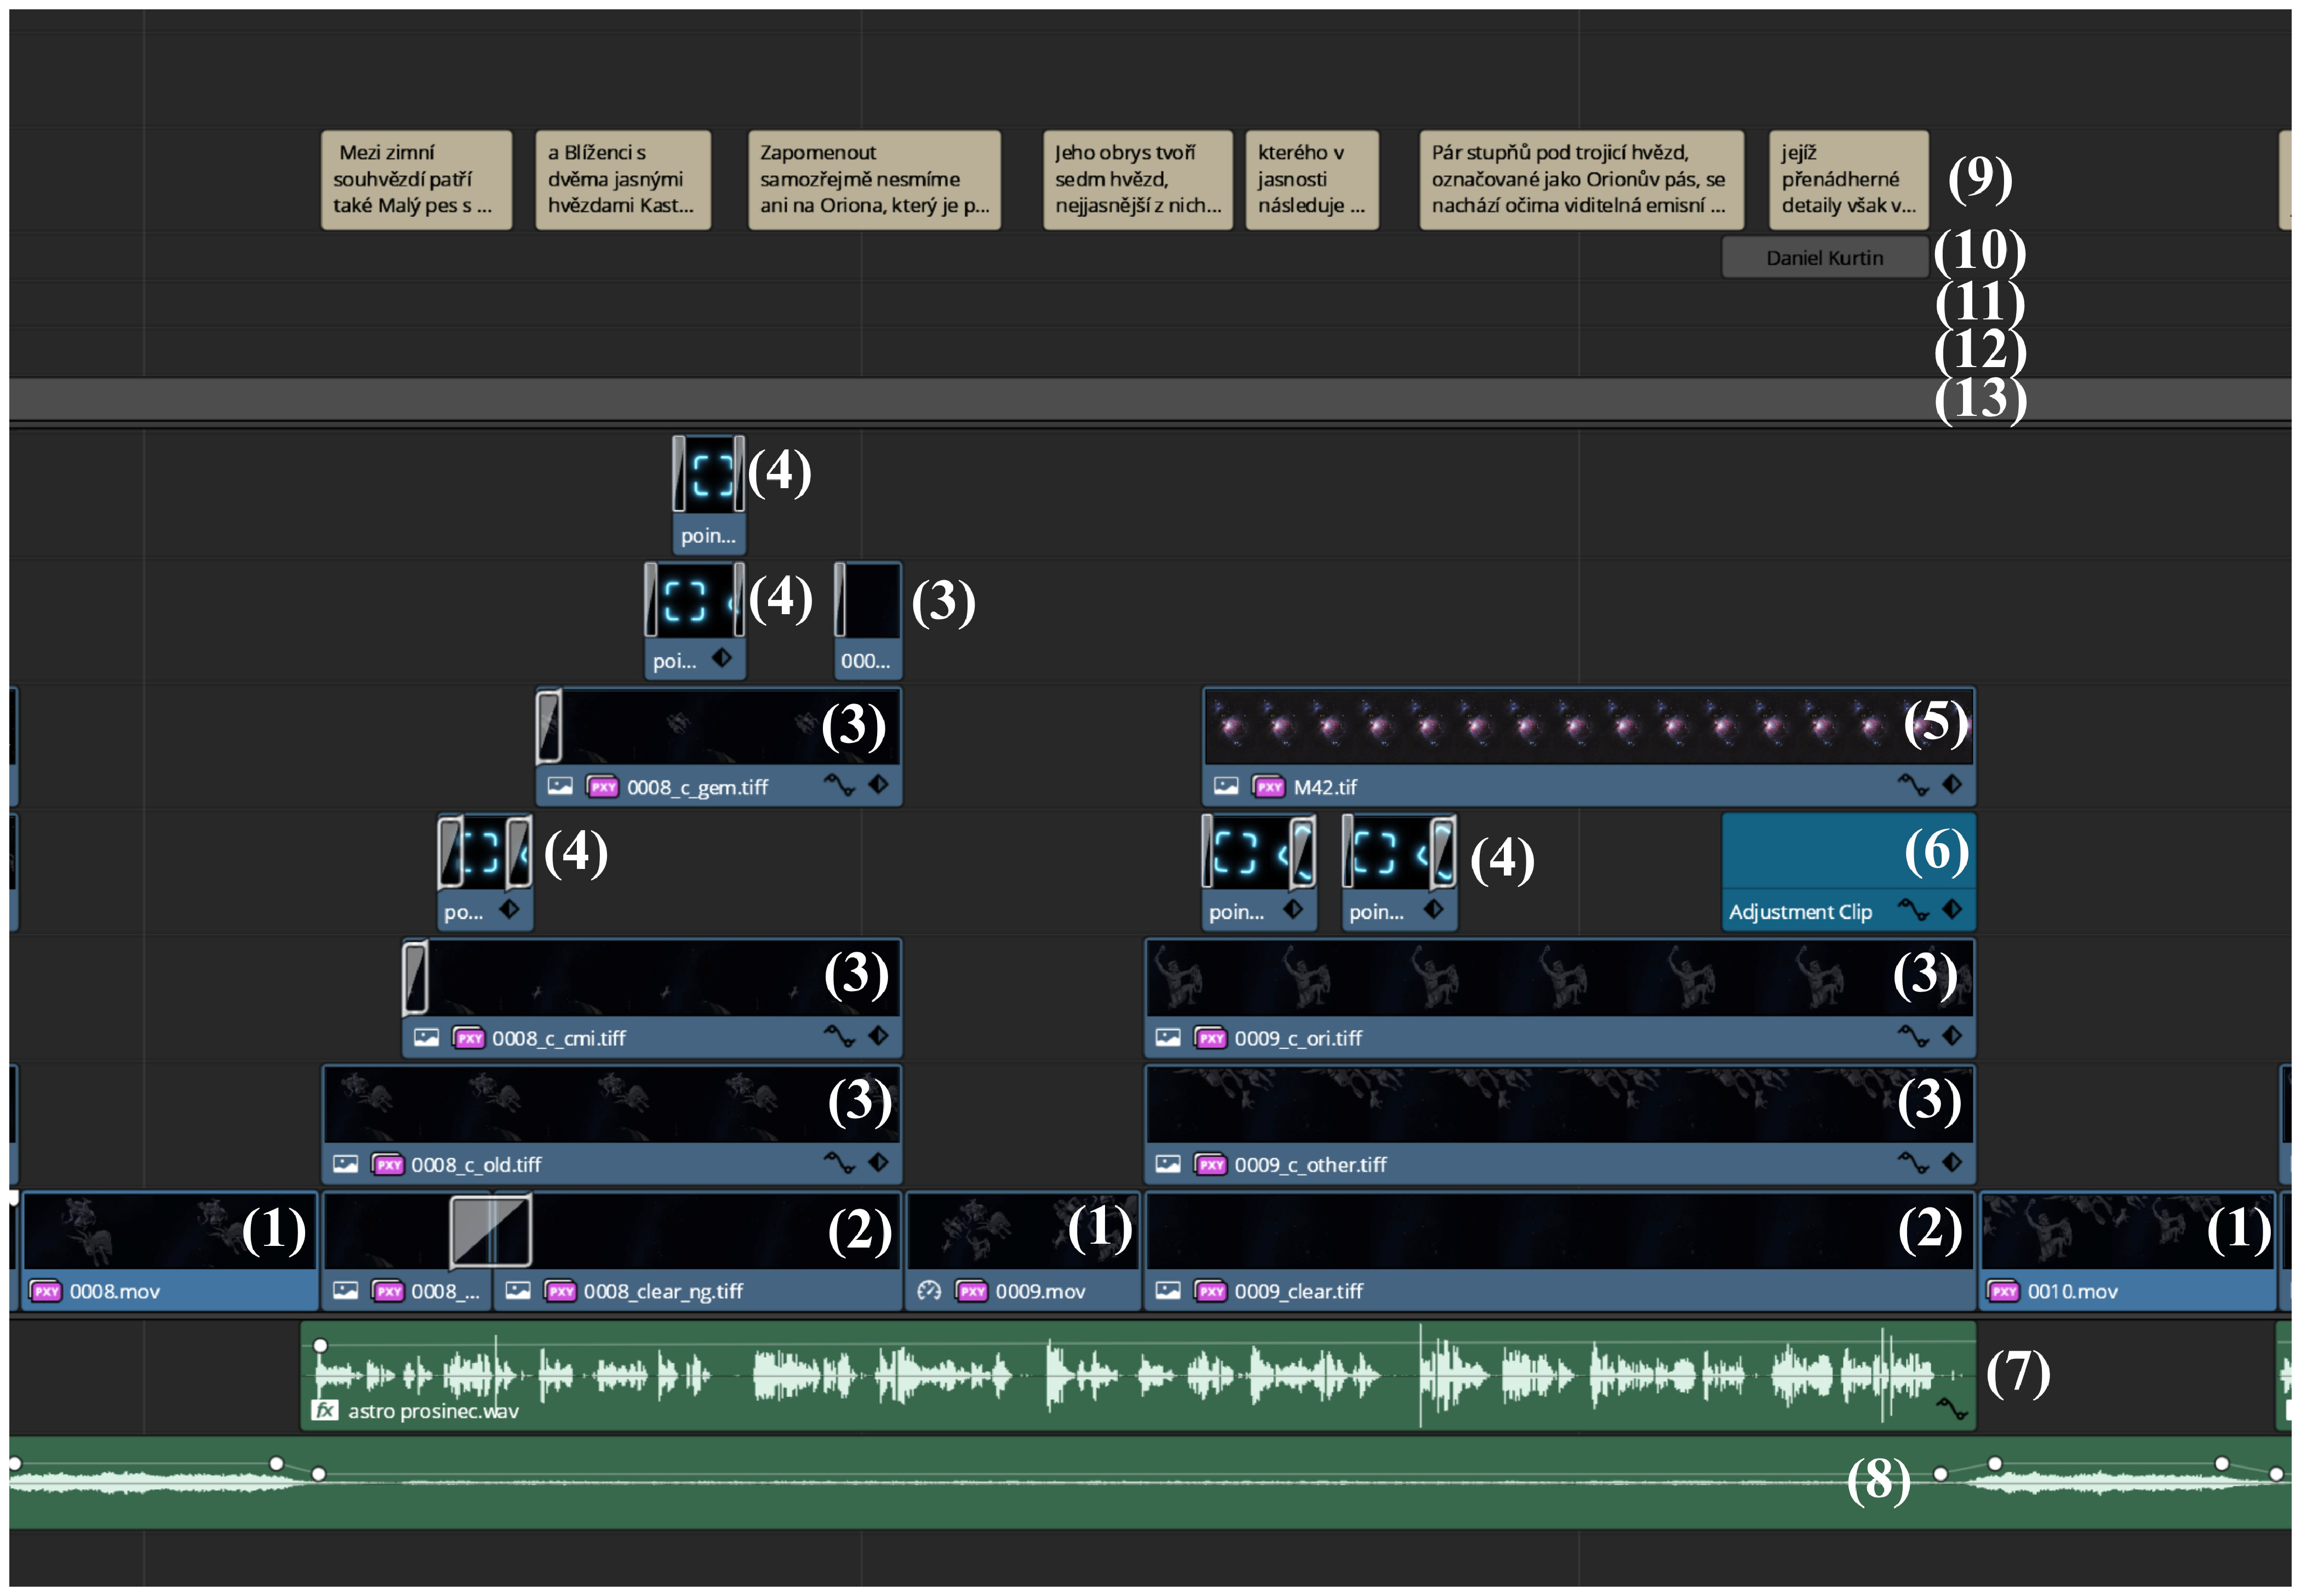
\includegraphics[width=1\textwidth]{timeline_annotated.eps}
	\caption{Snímek jedné ze scén z finálního videa. Každá důležitá stopa má přiřazené číslo. Vysvětleno v~oddílu~\ref{makingof:resolve:merging}}\label{img:timeline}
\end{figure}

\begin{figure}[H]
	\centering
	
\includegraphics[width=.5\textwidth]{pointer.eps}
	\caption{Animace zvaná pointer, využívaná pro upřesnění pozice objektu, o~kterém v~daném momentě mluví scénář.}\label{img:pointer}
\end{figure}

Nad scénou se nachází pět až šest stop s~titulky. Tyto stopy využíváme nejen pro standardní využití ve formě titulků v~Češtině a~někdy i~v Angličtině, ale využíváme je i~jako prostor pro citování zdrojů obrazových materiálů, opravě chyb v~již vydaném videu, poznámky a~doplnění obsahu od editora a~stopa s~informacemi a~zdrojích hudby. Tento postup využíváme hlavně kvůli jednoduchosti tvorby titulků a~možnosti tyto titulky skrýt a~nebýt jimi rušen. 

Souhvězdí a~objekty hlubokého vesmíru jsou řazeny podle nejlepšího času pozorování od západu slunce k~východu slunce. Poté nastává část, kde zmíníme nejdůležitější události, které v~průběhu měsíce nastávají. Na tomto místě zmiňujeme meteorické roje a~atmosférické i~vesmírné úkazy, které se mohou v~průběhu měsíce ukázat.
\subsubsection{Mixování obrazové části}
Záběry jsou vrstveny přes sebe pomocí metody Lighten. Tato metoda pro každý pixel vypočítá barvu podle rovnice $[\max(r_1, r_2), \max(g_1, g_2), \max(b_1, b_2)]$,\fcite{wiki:blend} kde tato množina představuje červený, zelený a~modrý kanál v~tomto pořadí. Toto umožňuje světlým obrázkům souhvězdí překrývat se, aniž by bylo třeba odstraňovat u~každého pozadí. Tento způsob mixování také využívám pro fotografie objektů hlubokého vesmíru. 

Nejdříve získám obrázek daného objektu z internetu. Nejčastějším zdrojem je Wikipedie, která poskytuje jasné licenční podmínky. Pokud na Wikipedie nemá vhodný nebo dostatečně kvalitní obrázek, začnu hledat po internetu další fotografie. Občas ani tento krok nepomůže, zvláště u~objektů nezajímavých pro focení. V~tomto případě se otočím na celooblohové sady dat, například Digitized Sky Survey 2 nebo Mellinger color optical survey které získávám z Centra astronomických dat univerzity ve Štrasburku díky jejich nástroji Aladin. Tyto sady dat pokrývají značný zlomek celé oblohy a~z geografické pozice České republiky pokrývají 100\% viditelné oblohy. Tyto fotografie následně upravuji pomocí software Zoner Photo Studio X, kde upravím kontrast pozadí tak, aby bylo absolutně černé a~tudíž při kompletaci zmizelo. Následně odstraním hvězdy blízko okraje snímku, aby byl přechod mezi snímkem a~pozadím méně znatelný. Tyto fotografie jsou následně překrývány přes souhvězdí a~pozadí. 
\subsection{Mixování zvukové části}
Ve zvukové části jsou na sebe navrstveny stopy hudby a~hlasu. Hudbu jsem vlastnoručně vybíral ze seznamu hudby v~knihovně YouTube a~ze seznamu skladeb, využívaných softwarem SpaceEngine. Základním kritériem je, aby hudba nijak diváka nerušila ale zároveň pomáhala s~atmosférou celého videa. Jako úvodní hudbu v~našich videích používáme stopu \textit{Beyond --- Patrick Patrikios} ze zvukové knihovny YouTube. V~hlavní části se objevují stopy z software SpaceEngine, jako například \textit{Space G Lydian --- Alfred Potter}, \textit{The Blithering Heights --- Akira} a~\textit{A peaceful Place --- Goodstreet}. Jako naší koncovou hudbu využíváme stopu \textit{Instant Crush --- Corbyn Kites} znovu ze Zvukové knihovny YouTube.
\section{Historie popularizace astronomie (WIP)}

\section{Historie a~vývoj procesu tvorby astronomických videí}
Proces tvorby našich astronomických videí se v~průběhu let výrazně změnil. První video jsme vytvořili v~roce 2021 a~od té doby jich vzniklo dalších 10\footnote{Započítávám zatím nevydaná videa, která budou vydaná do data maturitních zkoušek}.V této části se podíváme na celou historii tvorby astronomických videí skupinou AstroCrew.
\subsection{Začátky --- Prosinec 2021}
Naše cesta začala v~prosinci roku 2021. Zde jsme 14.\ prosince vydali naše první video. Toto video nebylo primárně určené k~vydání na platformě YouTube ale bylo připraveno pro planetárium v~iQLandii, kde jsme ho představili již 9.\ prosince. Celé video je kvůli tomu promítnuto sféricky, jak můžete vidět na obrázku~ref{img:prosinec}. Pro YouTube jsme toto video modifikovali, aby ho YouTube vzal jako 360° video, i~když polovina videa je čistě černá. Co se týče produkce, toto video bylo velice náročné. Stříhací program, kterým byl v~té době ještě Adobe Premiere Pro, neustále padal, a~obecně tvorba animací v~té době probíhala ještě manuálně. Stellárium dává k~dispozici webové rozhraní umožňující plnou kontrolu nad danou instancí Stellária. 

Toto video jsem natáčel tak, že jsem namířil Stellarium podobně, jako je namířená kopule planetária v~iQLandii a~poté jsem pomocí přesouvání času přemisťoval souhvězdí a~jednotlivé objekty tak, aby byly co nejlépe vidět. Následně jsem pomocí programu Adobe After Effects vložil do scény obrázky daných objektů hlubokého vesmíru pomocí integrovaného efektu VR Converter. Díky technologii Adobe Dynamic Link jsem poté jen vložil kompozice z After Effects přímo do časové osy v~Premiere Pro a~nemusel jsem je exportovat. Bohužel tento přístup je neskutečně pomalý a~snižuje významně výkonnost celého stříhacího programu. Z tohoto důvodu je Prosinec 2021 jediným videem vytvořeným v~tomto stylu.

\begin{figure}[ht]
	\centering
	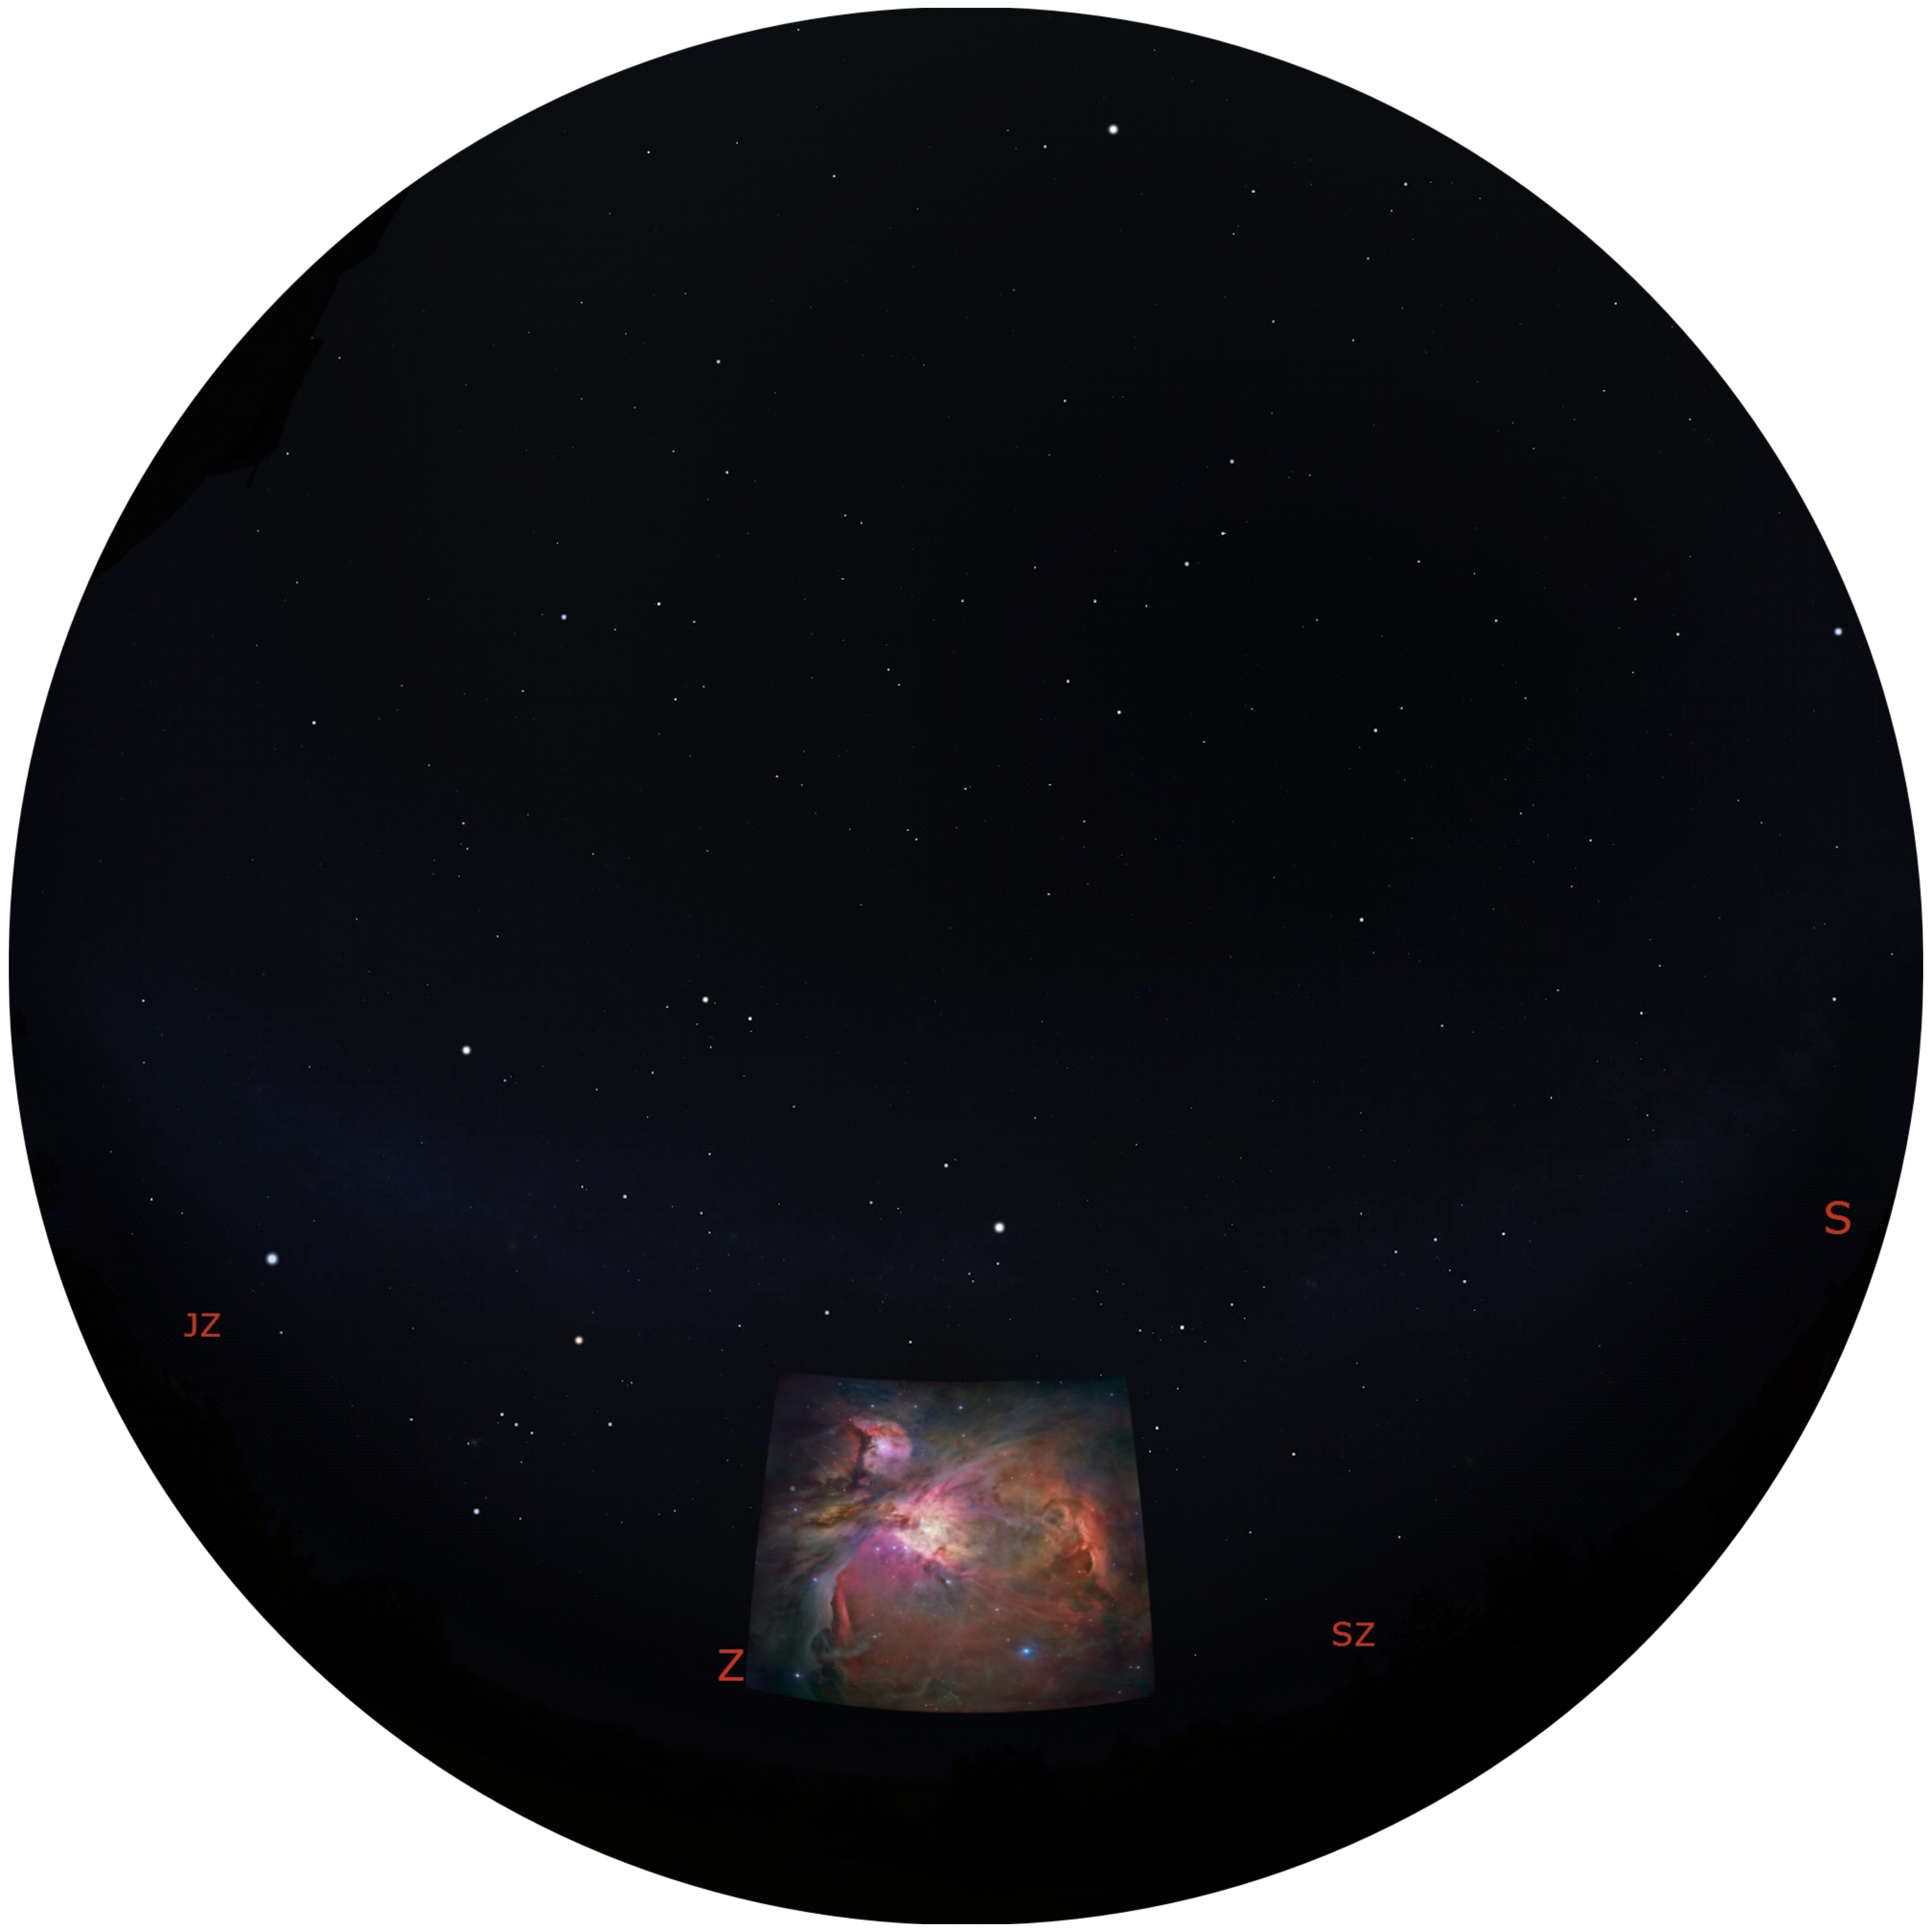
\includegraphics[width=.7\textwidth]{prosinec.eps}
	\caption{Demonstrace našeho prvního videa.}\label{img:prosinec}
\end{figure}
\subsection{Jednoduchá éra --- Březen až Květen 2022}
Celý proces, jak jsem ho popsal v~sekci~\ref{makingof} je aktuálním stavem tvorby. Na úplném začátku produkce tento proces ještě neexistoval a~veškeré znalosti potřebné pro tvorbu \textquote{moderních} videí bylo nutné získat postupným experimentováním. Videa v~této éře byla velice jednoduchá. Animace byly vytvořeny nahráváním okna Stellaria a~jeho ovládáním přes webové rozhraní. 

Ačkoliv tento proces byl jednoduchý na provedení, byl náročný na čas. Pokud jsem vybral špatný objekt, musel jsem se vrátit na předchozí a~nahrát celý přechod znovu. Pokud se Stellarium trochu zaseklo někde uprostřed přechodu, musel jsem daný přechod nahrát znovu. Tyto situace se mohou zdát nedůležité, ale při množství přechodů, které v~té době ve videích byly, se tyto časové ztráty jednoduše nasčítaly a~zpomalily celou produkci videa. Ukázku finálního videa jsem připojil v~přílohách jako obrázek~\ref{img:brezen}.

Do této kategorie se připletlo ještě video s~názvem \textquote{Jak pozorovat zatmění Měsíce 16.5.2022}, které jsme vydali 13. 5. 2022. Toto video je přechodem k~další éře, primárně z důvodu, že neobsahuje ani jeden záběr ze Stellaria. Toto video se skládá primárně ze záběrů zatmění měsíce a~animace vygenerované pomocí systému Space Engine. Ačkoliv toto video má největší počet shlédnutí na našem YouTube kanálu, má relativně nízký dopad na náš YouTube kanál, jelikož většina těchto shlédnutí je ze stránek astro.cz a~seznamzpravy.cz, na které toto video nasdílel Martin Gembec, vedoucí planetária v~iQLandii.
\begin{figure}[ht]
	\centering
	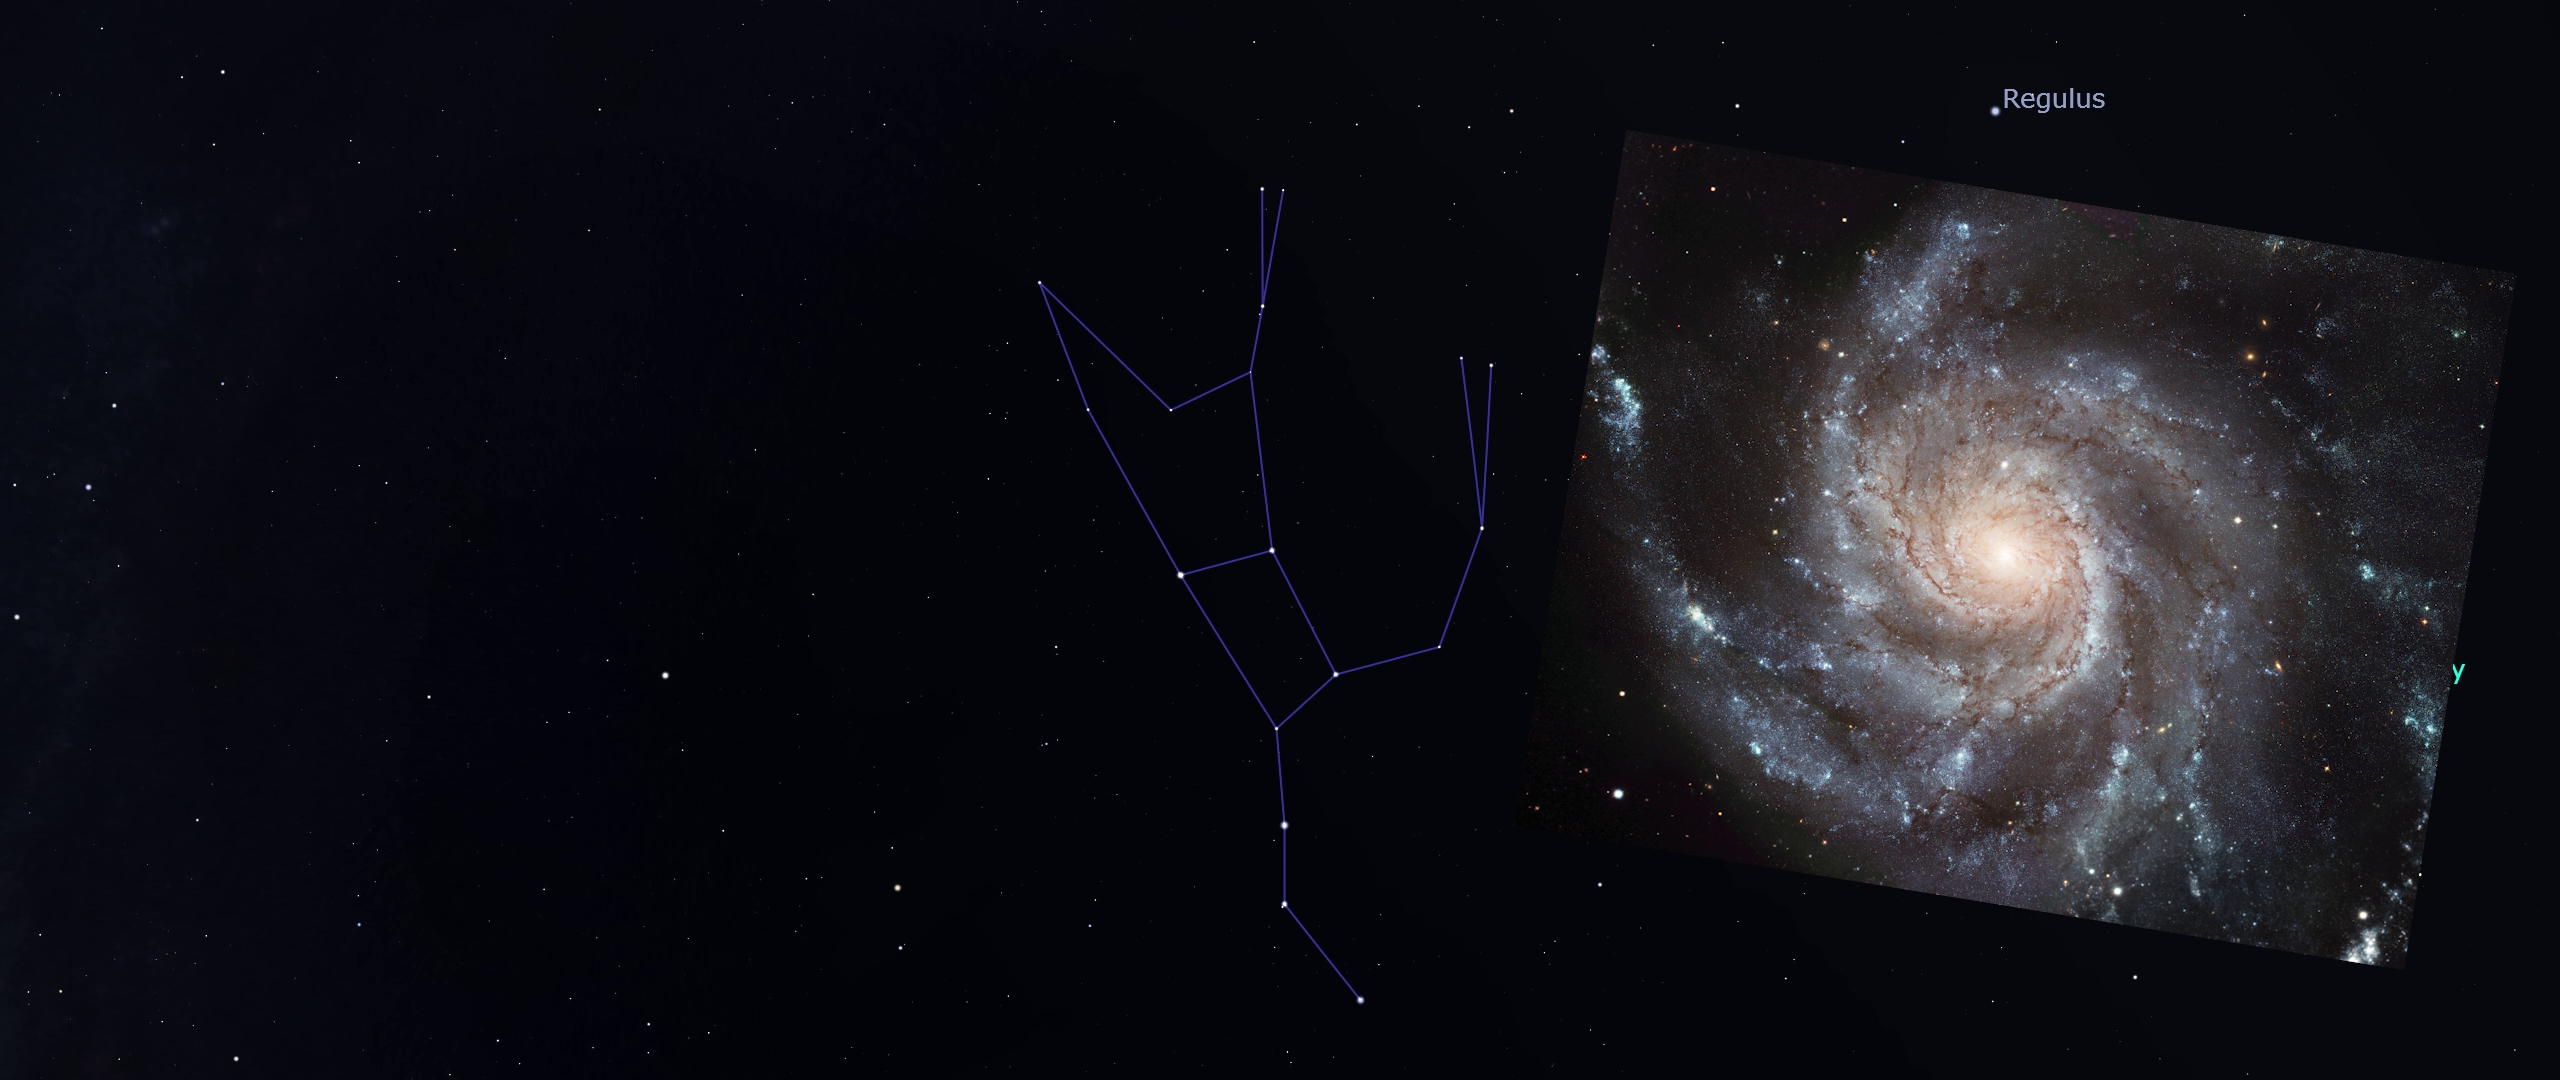
\includegraphics[width=.85\textwidth]{brezen.png}
	\caption{Demonstrace našeho prvního videa.}\label{img:brezen}
\end{figure}
\subsection{Éra spěchu --- Červen a~Červenec 2022}
Červnové a~červencové Astronomické desetiminutovky byly stříhány ve velikém spěchu. S~příchodem prázdnin se množství volného času, který jsem měl k~dispozici na stříhání se snížilo a~tudíž bylo třeba produkci optimalizovat. V~této době jsem také začal přecházet do nového stříhacího programu, zvaného DaVinci Resolve, který využívám doteď. Tato změna prostředí produkce znamenala, že videa musela být jednodušší na produkci a~tudíž kvalita lehce upadla. Ukázku finálního videa jsem připojil v~přílohách jako obrázek~\ref{img:cervenec}.

Tato videa jsou jednoduchá, složená z časosběrných záběrů se zvukovým komentářem a~občasnými grafikami, vytvořenými ručně ve Stellariu. Tato videa jsou opravdu základní a~rád bych je v~budoucnu znovu navštívil a~pokusil se je předělat na moderní formát. Nicméně tato videa sloužila jako můstek k~modernímu procesu tvorby videí, který se poprvé projevil v~Únorových Astronomických desetiminutovkách.

\begin{figure}[ht]
	\centering
	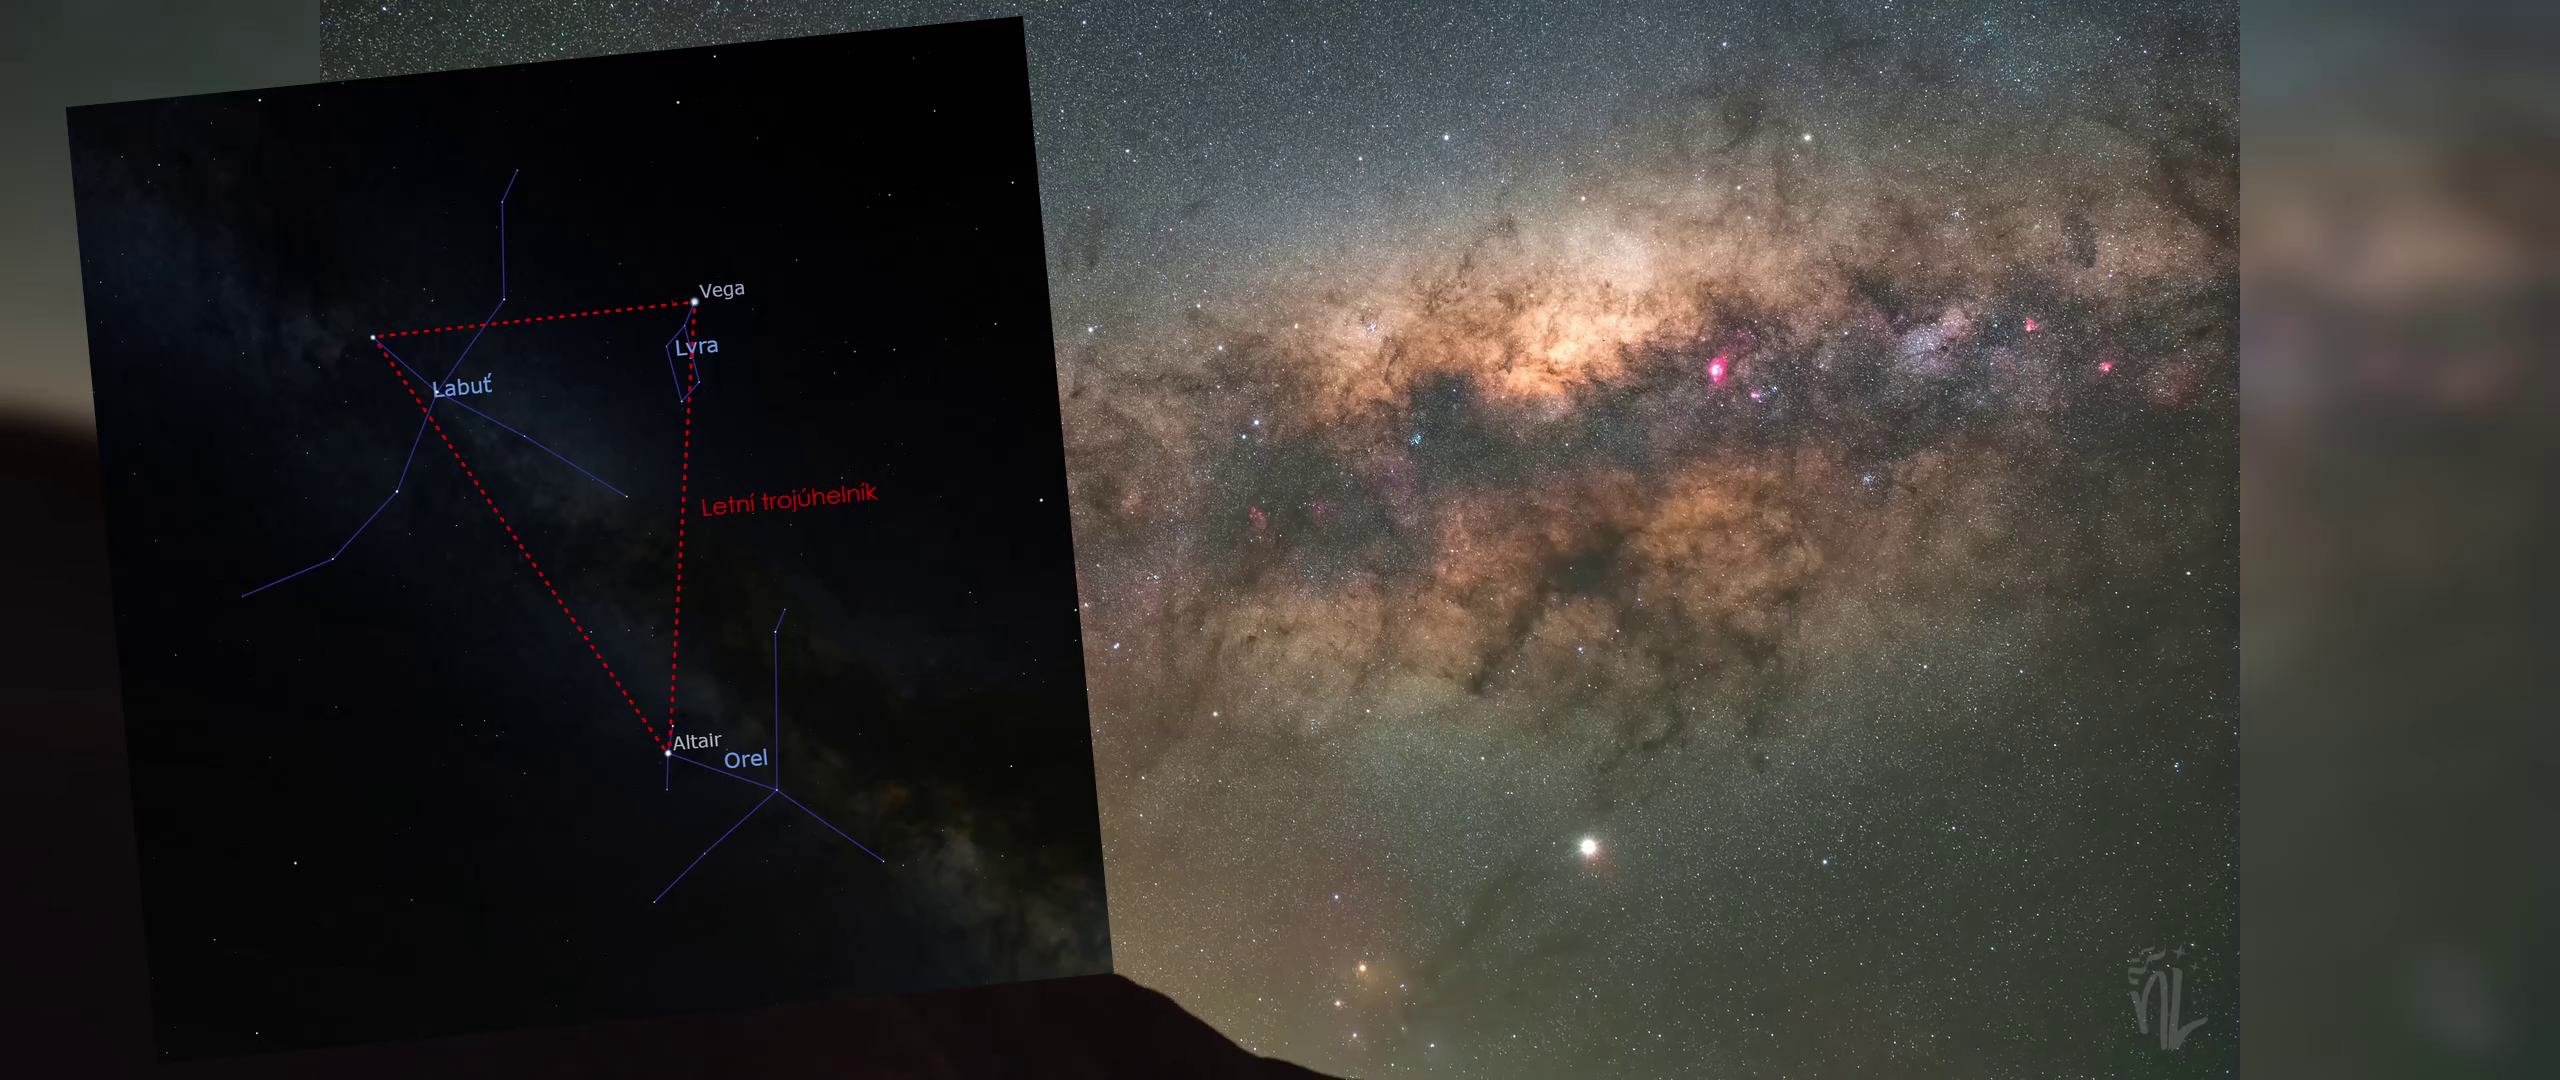
\includegraphics[width=.85\textwidth]{cervenec.png}
	\caption{Demonstrace našeho prvního videa.}\label{img:cervenec}
\end{figure}
\subsection{Renezance Astrocrew --- Únor 2023}
První video, které se dá kategorizovat pod skupinu moderních AstroCrew videí. V~této době jsem poprvé začal pracovat se Stellariem jako s~nástrojem pro generování dat, která jsou později upravena do finální podoby místo jeho využívání jako zdroj videa. 

Základní metodika byla jednoduchá, nafotit celooblohovou panorámu oblohy, složit jí do jednoho snímku a~ten poté otáčet ve stříhacím programu. V~této době začal vznikat nástroj StellariumPanoramaCreator (dále jen jako SPC), který se již v~produkci udržel. První verze SPC byla velice jednoduchá. Skript převzal kontrolu nad klávesnicí a~myší mého počítače a~pomocí integrovaného okna přímo ve Stellariu, které umožňovalo zadat azimut a~výšku, postupně nafotilo všech 54 panelů, ze kterých se poté finální panoráma složila za pomoci programu Hugin, který dostal všechny panely a~projektový soubor, který byl vygenerován při běhu SPC.\@ Následně Hugin převedl tyto panely do kompletní panorámy.

Zpracování těchto dat bylo mnohem komfortnější než skládání videí natočených manuálně ale pořád vyžadovalo mnoho práce, než byla data získána a~tento čas nebylo možné nijak jinak využít. Během získávání dat nebylo možné využívat ani klávesnici ani myš. Nebylo možné ani odkliknout z okna, jelikož pro ovládání Stellaria bylo třeba, aby Stellarium zachytávalo klávesnici i~myš. Proto dalším logickým krokem bylo převedení komunikace za oponu. 

Ideálním řešením se ukázalo být webové rozhraní Stellaria. Tento modul je určen pro řízení Stellaria z tabletu nebo jiného počítače v~případě, že není možné ovládat počítač se Stellariem. Na pozadí tento systém využívá architektury HTTP, která umožňuje přistupovat k~specifickým částem kódu Stellaria přes lokální síť. Tento modul byl vyvinut jako projekt v~rámci akce \textquote{ESA Summer of Code 2015}\fcite{stellarium:rcDoc}. 

Dokumentace\fcite{stellarium:rcAPI} tohoto protokolu je bohužel v~některých místech relativně chaotická a~nečitelná. Pro vývoj jsem tedy použil existující HTML rozhraní a~pomocí vývojářských nástrojů, dostupných ve většině moderních prohlížečů, jsem postupně zjistil veškeré adresy a~parametry, které mám Stellariu posílat, aby dělalo to, co má. Poté jsem SPC přepsal, aby místo ovládání klávesnice a~myši využívalo nově dostupné HTTP dotazy. Po náročné optimalizaci načasování jednotlivých příkazů se časová náročnost snížila přibližně na polovinu předchozího času a~celý proces mohl nyní proběhnout na pozadí. Ukázku finálního videa jsem připojil v~přílohách jako obrázek~\ref{img:unor}.

V této fázi střih probíhal zpět v~Adobe Premiere Pro, primárně kvůli pluginu Gopro FX Reframe, který panorámu, kterou jsem vygeneroval v~předchozím kroku, převedl na perspektivní zobrazení. Tento systém měl mnoho výhod oproti předchozímu procesu, při kterém bylo nutné perfektně trefit načasování při natáčení a~když se něco nepodařilo, bylo nutné celý segment natočit znovu. V~této verzi procesu stačilo přeanimovat poslední přechod a~upravit časování sekvence a~problém byl vyřešen. I~tak, tento postup nesl značné nevýhody. Hlavní z nich byla neskutečná zátěž systému, z části podpořena i~přirozená zátěž samotného Premiere. Tento fakt znamenal, že export Únorových Astronomických desetiminutovek zabral 90 minut na 12 minut videa. V~říjnu 2023 se navíc tento plugin kompletně rozpadl a~úplně přestal fungovat, což prakticky zrušilo Říjnové Astronomické desetiminutovky. Proto pro následující projekt bylo nutné vyvinout nový proces. 
\subsection{Moderní Astrocrew --- Rok 2024, Prosinec 2024 a~Rok 2025}
V listopadu roku 2023 přinesl Dan do naší skupiny nápad, udělat video, shrnující úkazy, které budou vidět v~následujícím roce na obloze. Po nedávném neúspěchu ve tvorbě Říjnových Astronomických desetiminutovek bylo nutné změnit celý proces. Prvním pokusem bylo využití animačního programu Blender a~zachování exportu panorám a~jejich pozdější přemapování do perspektivního zobrazení. Tento postup sice fungoval, ale při tvorbě jsem byl nucen každé video exportovat \(2\times \), jednou jako panorámu a~jednou jako animovaný přechod. Během pokusů s~touto metodou mě ale napadla revoluční myšlenka. Místo exportu celé panorámy, ze které jsem pokaždé minimálně polovinu zahodil, exportovat pouze potřebnou oblast pro finální video. 

V této epoše se StellariumPanoramaCreator (dále jen SPC) přetvořil do téměř finální podoby. Jako vstup sloužily souřadnice a~časy jednotlivých zastávek a~SPC následně ovládal Stellarium pomocí HTTP, jako v~předchozí edici. Výstupem bylo 500 snímků pro každý přechod v~rozlišení \(3840\times2160\) pro složení do finálního videa. Ačkoliv tento postup byl výrazně rychlejší a~příjemnější než postupy předchozí, odhalil také několik slabých stránek implementace webového rozhraní Stellaria. Stellarium je schopné z webu zpracovávat příkazy pouze sekvenčně, tudíž není možné odeslat všechny příkazy naráz a~jen počkat, než se Stellarium vzpamatuje, místo toho je nutné načasovat každý příkaz tak, aby strávil ve frontě minimum času.

Tímto způsobem bylo vytvořeno video \textquote{Co nás čeká na obloze v~roce 2024?}. Pro videa \textquote{Astronomické desetiminutovky --- Prosinec} a~\textquote{Co nás čeká na obloze v~roce 2025?} byla provedena malá změna, kdy se příkazy přestaly odesílat přes HTTP ale byly zapsány do skriptového souboru Stellaria, které následně tyto příkazy spustilo v~maximální dostupné rychlosti.
\begin{figure}[ht]
	\centering
	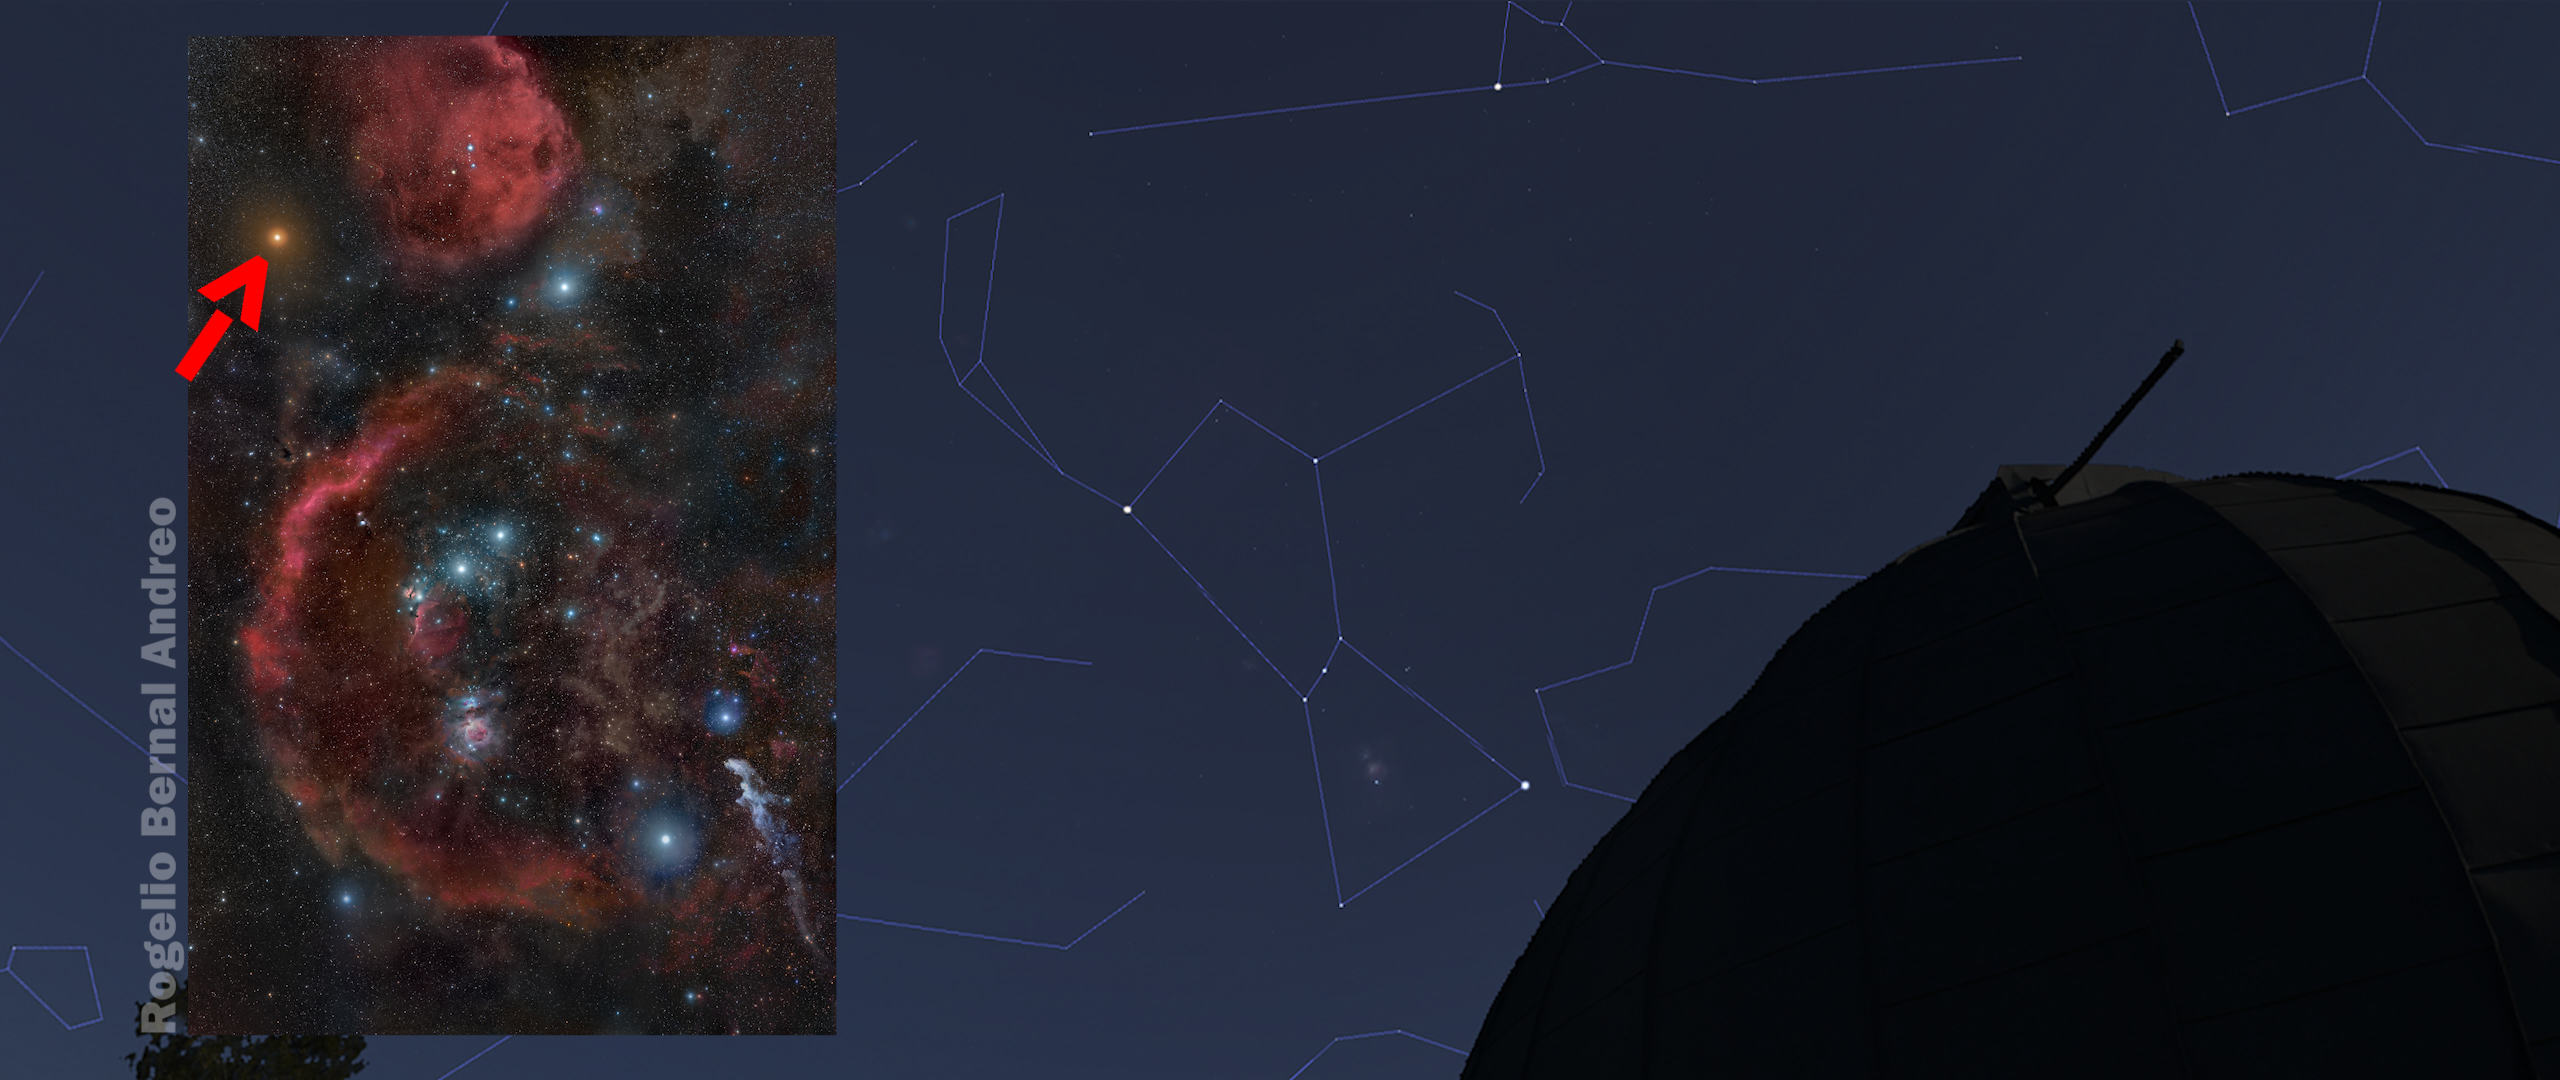
\includegraphics[width=.85\textwidth]{unor.png}
	\caption{Demonstrace našeho prvního videa.}\label{img:unor}
\end{figure}
\newpage
\part{Praktická část}
\section{Astronomické desetiminutovky --- Prosinec}
Prosincové video je druhé video na našem kanále, které bylo renderováno pomocí metody skriptování Stellaria a~první skriptované video ze série Astronomických desetiminutovek. S~sebou přineslo mnoho změn v~procesu animace, zvláště pak v~oblasti editování. 

U předchozího videa ze série Astronomických desetiminutovek jsem ještě využíval celooblohových panorám a~pluginu Gopro FX Reframe. Prosincové Astronomické desetiminutovky byly tudíž novým milníkem v~produkci.

Prvním momentem, kdy se celá produkce změnila byla scéna v~čase 2:55, kdy jsem potřeboval zvýraznit jedno ze souhvězdí (viz obrázek~\ref{prac:ac12_1}). V~předchozích videích jsem těchto efektů dosahoval pomocí maskování nepotřebných částí ve stříhacím programu. Takto jsem mohl vytvořit jeden snímek, který zachycoval všechna souhvězdí a poté je jednotlivě maskovat v editoru. Podobný postup jsem tedy využil i poté, co jsem se zbavil celooblohového fotografování

\begin{figure}[h]
	\centering
	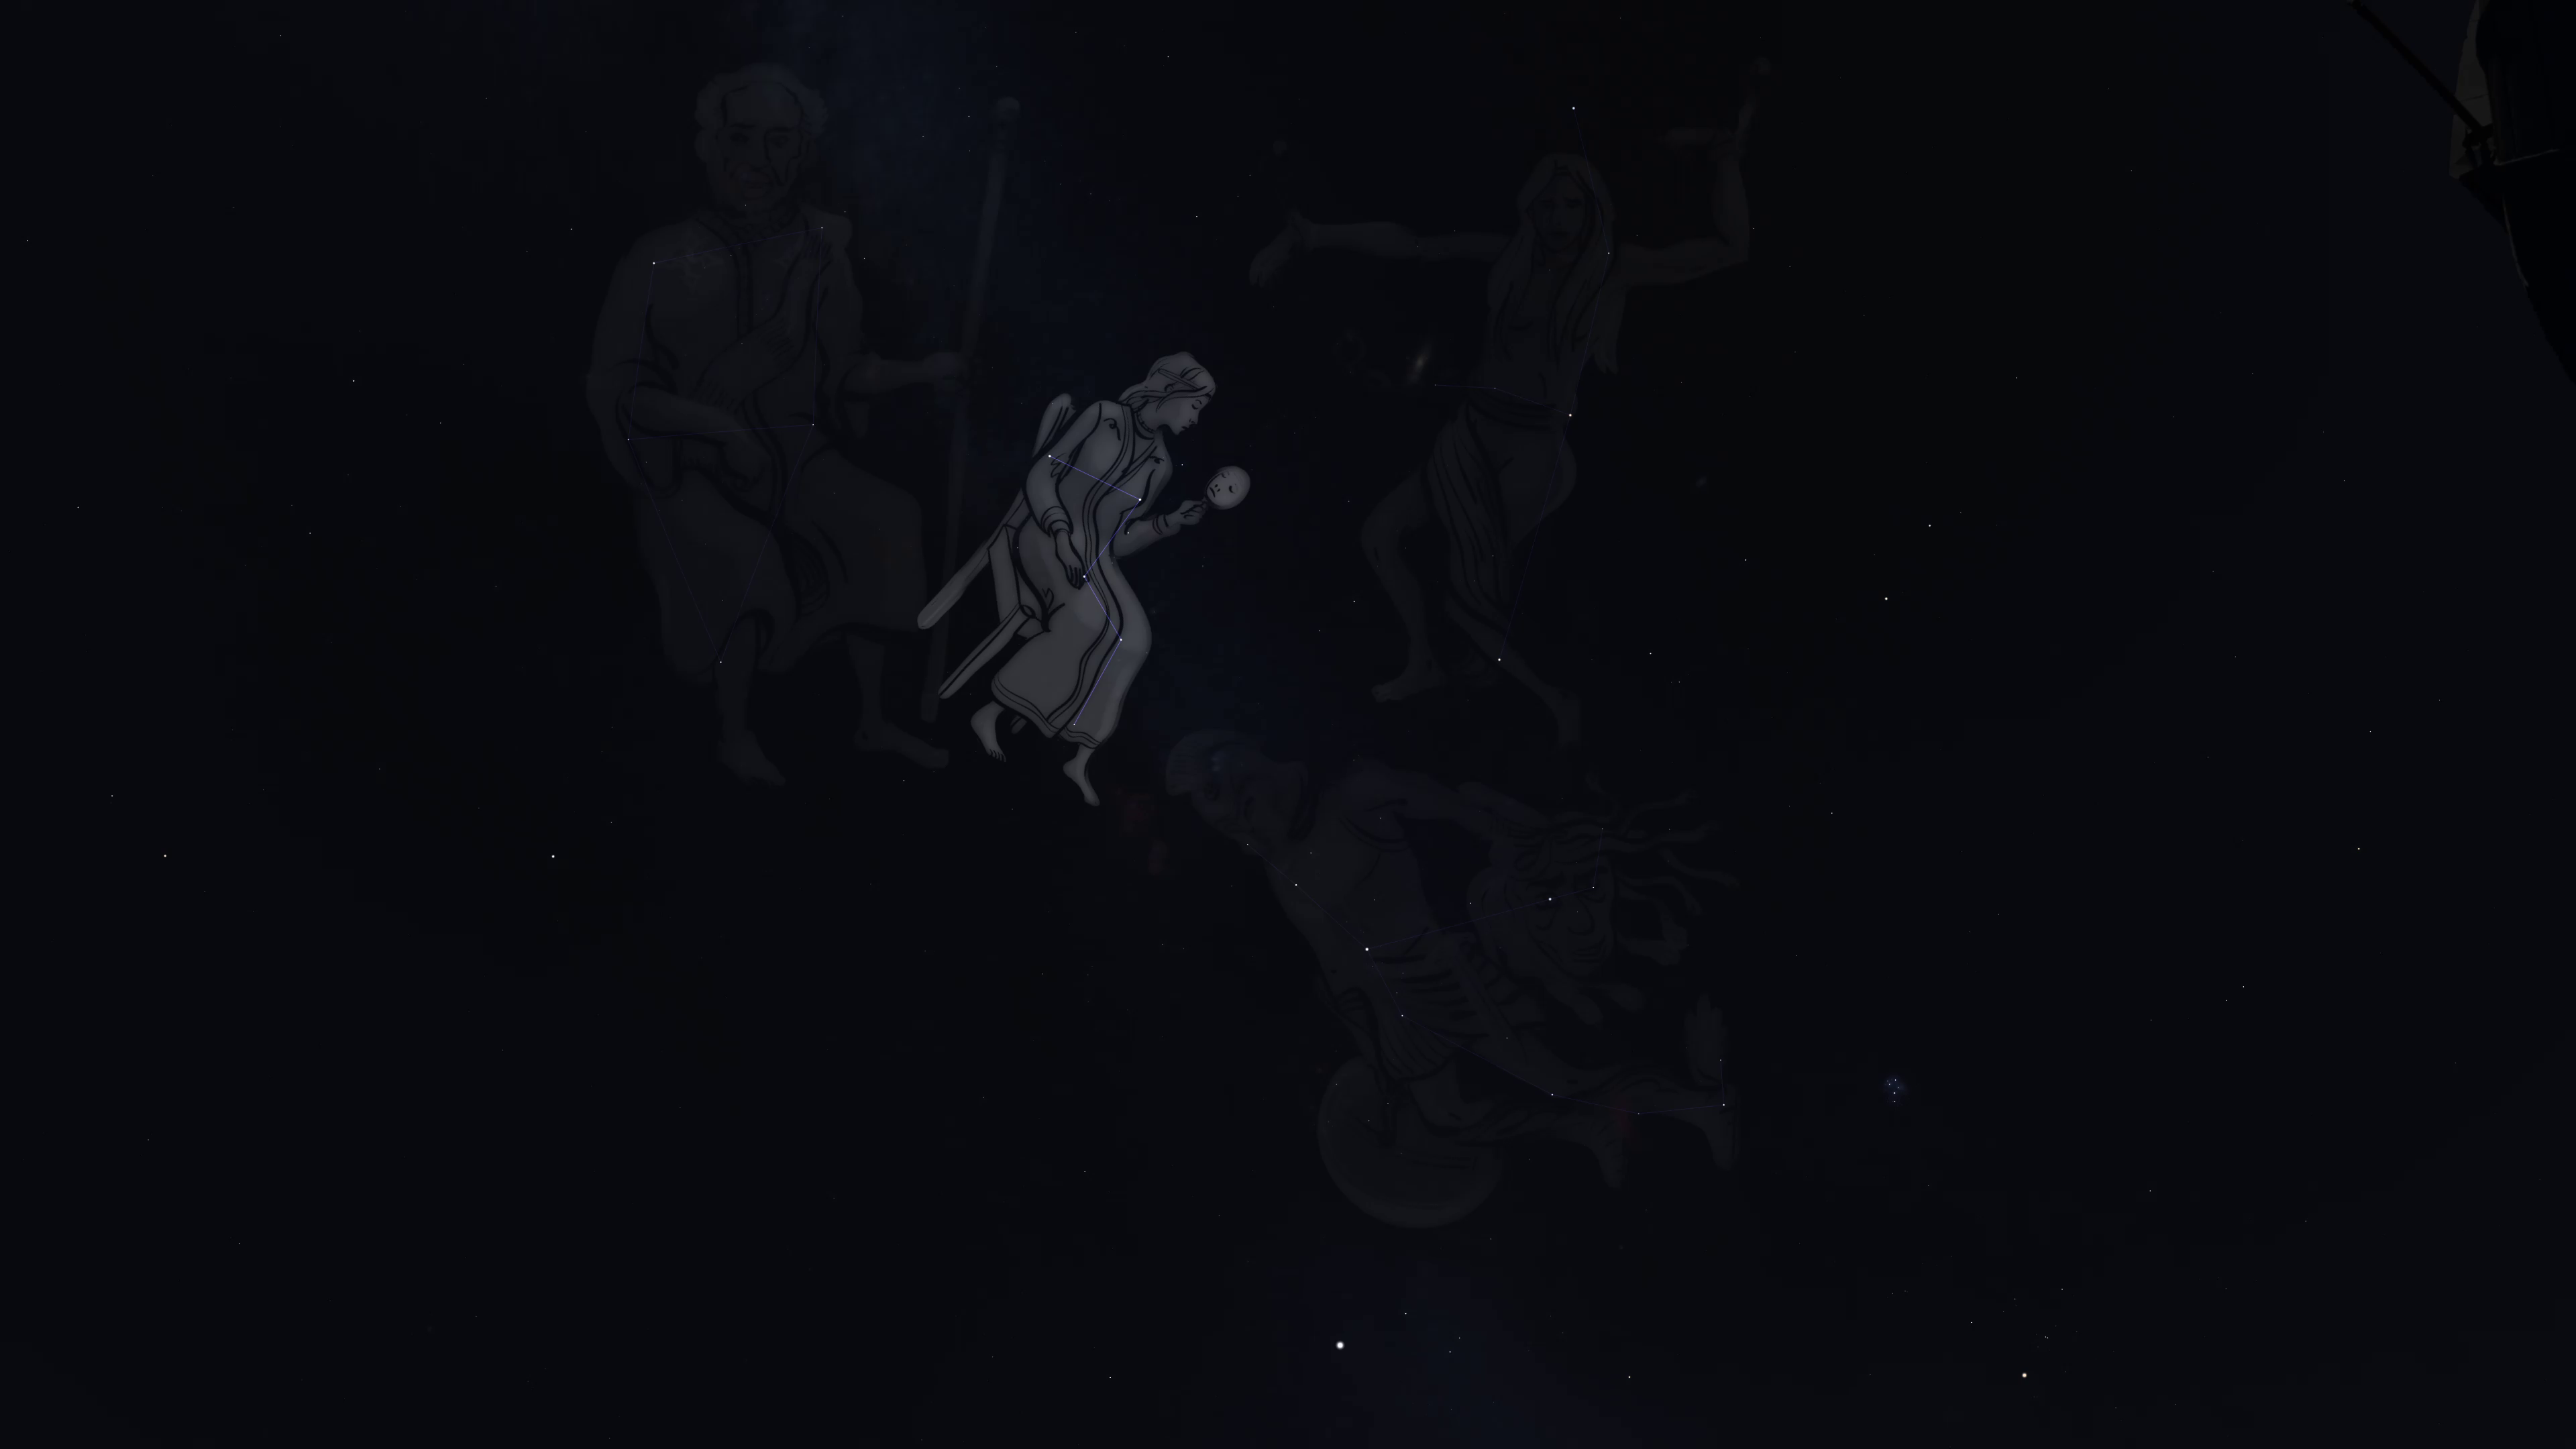
\includegraphics[width=.95\textwidth]{ac12_1.png}
	\caption{Demonstrace problematické scény z Prosincových Astronomických desetiminutovek.}\label{prac:ac12_1}
\end{figure}

Ačkoliv mi tento postup umožňoval větší kontrolu nad výsledným záběrem v editoru. Jeho nepraktičnost se ukázala v momentě, kdy jsem byl nucen scénu mírně pootočit kvůli chybě ve výpočtu data ve skriptu a byl jsem tedy nucen masku, kterou jsem již pečlivě naanimoval pro každé souhvězdí zvlášť během dalšího přechodu celou předělat.

V ten moment jsem se zamyslel, jestli by to nešlo udělat nějak lépe a napadlo mě, vyexportovat ze Stellaria jen potřebná souhvězdí a zbytek skrýt. Ukázalo se, že Stellarium má pro tento účel marker \textit{FlagIsolateSelected}, který umožní Stellariu renderovat pouze souhvězdí, která předem vyberu pomocí \textit{core.\-select\-Constellation\-By\-Name(name)}. Tato malá změna z pohledu diváka mi ušetřila nespočet hodin animování masek pro celé video. %chktex 36

Novinkou pro toto video byl také způsob zapracování objektů hlubokého vesmíru do jednotlivých záběrů. S tímto konceptem jsem si hrál i u zrušených říjnových Astronomických desetiminutovek, kde jsem dostal nápad, smíchat obrázky objektů hlubokého vesmíru s daty ze Stellaria. První snímek, který takto vznikl, můžete vidět jako obrázek~\ref{prac:ac12_2}. 

\begin{figure}[h]
	\centering
	\includegraphics[width=.95\textwidth]{ac12_2.png}
	\caption{První snímek s mixovanými objekty hlubokého vesmíru a dat ze stellaria, zpracování: Zoner Photo Studio X.}\label{prac:ac12_2}
\end{figure}

Tohoto efektu dosáhneme pomocí míchání metodou Lighten, kde zvolíme nejjasnější barvu každého pixelu z vrstev níže. Vstupní snímky, pokud se nejedná o snímky kulových hvězdokup, nejdříve zpracuji pomocí Starnet++, který ze snímků odstraní hvězdy. Následně vyčistím pozadí daného snímku, aby bylo co nejtmavší, jak je to možné. Tuto část snímku chceme odstranit a proto potřebujeme, aby ji metoda Lighten nikdy nevybrala, proto se snažím zajistit, aby měly tyto pixely co nejtmavší barvu. Následně do snímku vrátím některé hvězdy, které nezasahují do pozadí (Například u snímku~\ref{prac:ac12_2} bílého trpaslíka uprostřed mlhoviny).

Poslední krok je zarovnání snímku na místo, kde se na obloze nachází v realitě a pomalé prolnutí, využívající neschopnosti diváka všimnout si pomalých změn.

Tento typ zpracování obrázků dostal podporu od zbytku týmu a nyní ho využíváme pro většinu objektů hlubokého vesmíru.
\end{document}
